% Research report, EPSRC DLA project S3.5-COM-Valentino (University of Sheffield).
% Format: IEEEtran conference, mirroring the ICRA template preamble (letterpaper, 10pt, helvet, cite).
% Build:  cd docs/proposal && latexmk -pdf proposal.tex      Check:  pdfinfo proposal.pdf  ->  Pages: 3 at most
% Structure: Abstract (from the literature in docs/paper) -> Introduction -> Method -> Results -> Conclusion.
% Numbers come only from README.md; citations only from docs/paper/ and
% research_notes/Neurosymbolic world models proposal/ (verified earlier).
\documentclass[letterpaper, 10pt, conference]{IEEEtran}
\IEEEoverridecommandlockouts
\usepackage{amsmath,amssymb}
\usepackage{graphicx}
\usepackage{booktabs}
\usepackage{array}
\usepackage{xcolor}
\usepackage{cite}
\usepackage{capt-of}
\usepackage[hidelinks]{hyperref}
\usepackage[scaled=0.92]{helvet}
\setlength{\textfloatsep}{8pt plus 2pt minus 2pt}
\setlength{\dbltextfloatsep}{8pt plus 2pt minus 2pt}
\setlength{\floatsep}{7pt plus 2pt minus 2pt}
\graphicspath{{../images/}}
\AtBeginDocument{\setlength{\abovedisplayskip}{2pt}\setlength{\belowdisplayskip}{2pt}}
\renewcommand{\topfraction}{0.9}\renewcommand{\dbltopfraction}{0.9}
\renewcommand{\textfraction}{0.07}\renewcommand{\floatpagefraction}{0.9}

\newcommand{\applicant}{Ned Pham}   % <- check spelling, then rebuild
\newcommand{\demourl}{https://neural-symbolic-nlp.onrender.com/train-neural-symbolic}
\newcommand{\codeurl}{https://github.com/nhan03bit/neural_symbolic_nlp}

% Header box (as in the ICRA template): abstract and index terms left, Fig. 1 right.
% The abstract summarises the literature in docs/paper, not the implementation.
\definecolor{absgray}{gray}{0.92}
\newcommand{\abstracttext}{Neural networks trained by next-word prediction are strong at perception, but keep no explicit link to the rules behind a decision. Sheth, Roy and Gaur argue that safety-critical AI needs knowledge set as guardrails during training, not after it, and sort neurosymbolic methods into \emph{lowering}, which compresses symbolic knowledge into the network, and \emph{lifting}, which maps neural outputs to symbols for reasoning. On the lowering side, the semantic loss of Xu et al.\ turns a logical constraint into a training term. Ahmed et al.\ extend it to autoregressive models, where the exact probability of a constraint is \#P-hard, and on GPT-2 pair it with word banning at decoding. A loss gives no test-time guarantee, and a mask leaves the model unchanged. This report asks what happens when one knowledge base drives both and a verifier lifts the output back to symbols, on a small transformer, and proposes the same split for neurosymbolic world models in robotic manipulation.}
\makeatletter
\let\old@maketitle\@maketitle
\renewcommand{\@maketitle}{\old@maketitle\vspace{-4pt}\setcounter{figure}{0}
\noindent\colorbox{absgray}{\begin{minipage}{\dimexpr\textwidth-2\fboxsep\relax}
\begin{minipage}[c]{0.445\linewidth}\sffamily\small\bfseries
\textit{Abstract}---\abstracttext\par\smallskip
\textit{Index Terms}---Neuro-symbolic AI, lowering and lifting, semantic loss, constrained decoding, knowledge bases, world models, robotic manipulation.
\end{minipage}\hfill
\begin{minipage}[c]{0.535\linewidth}\centering
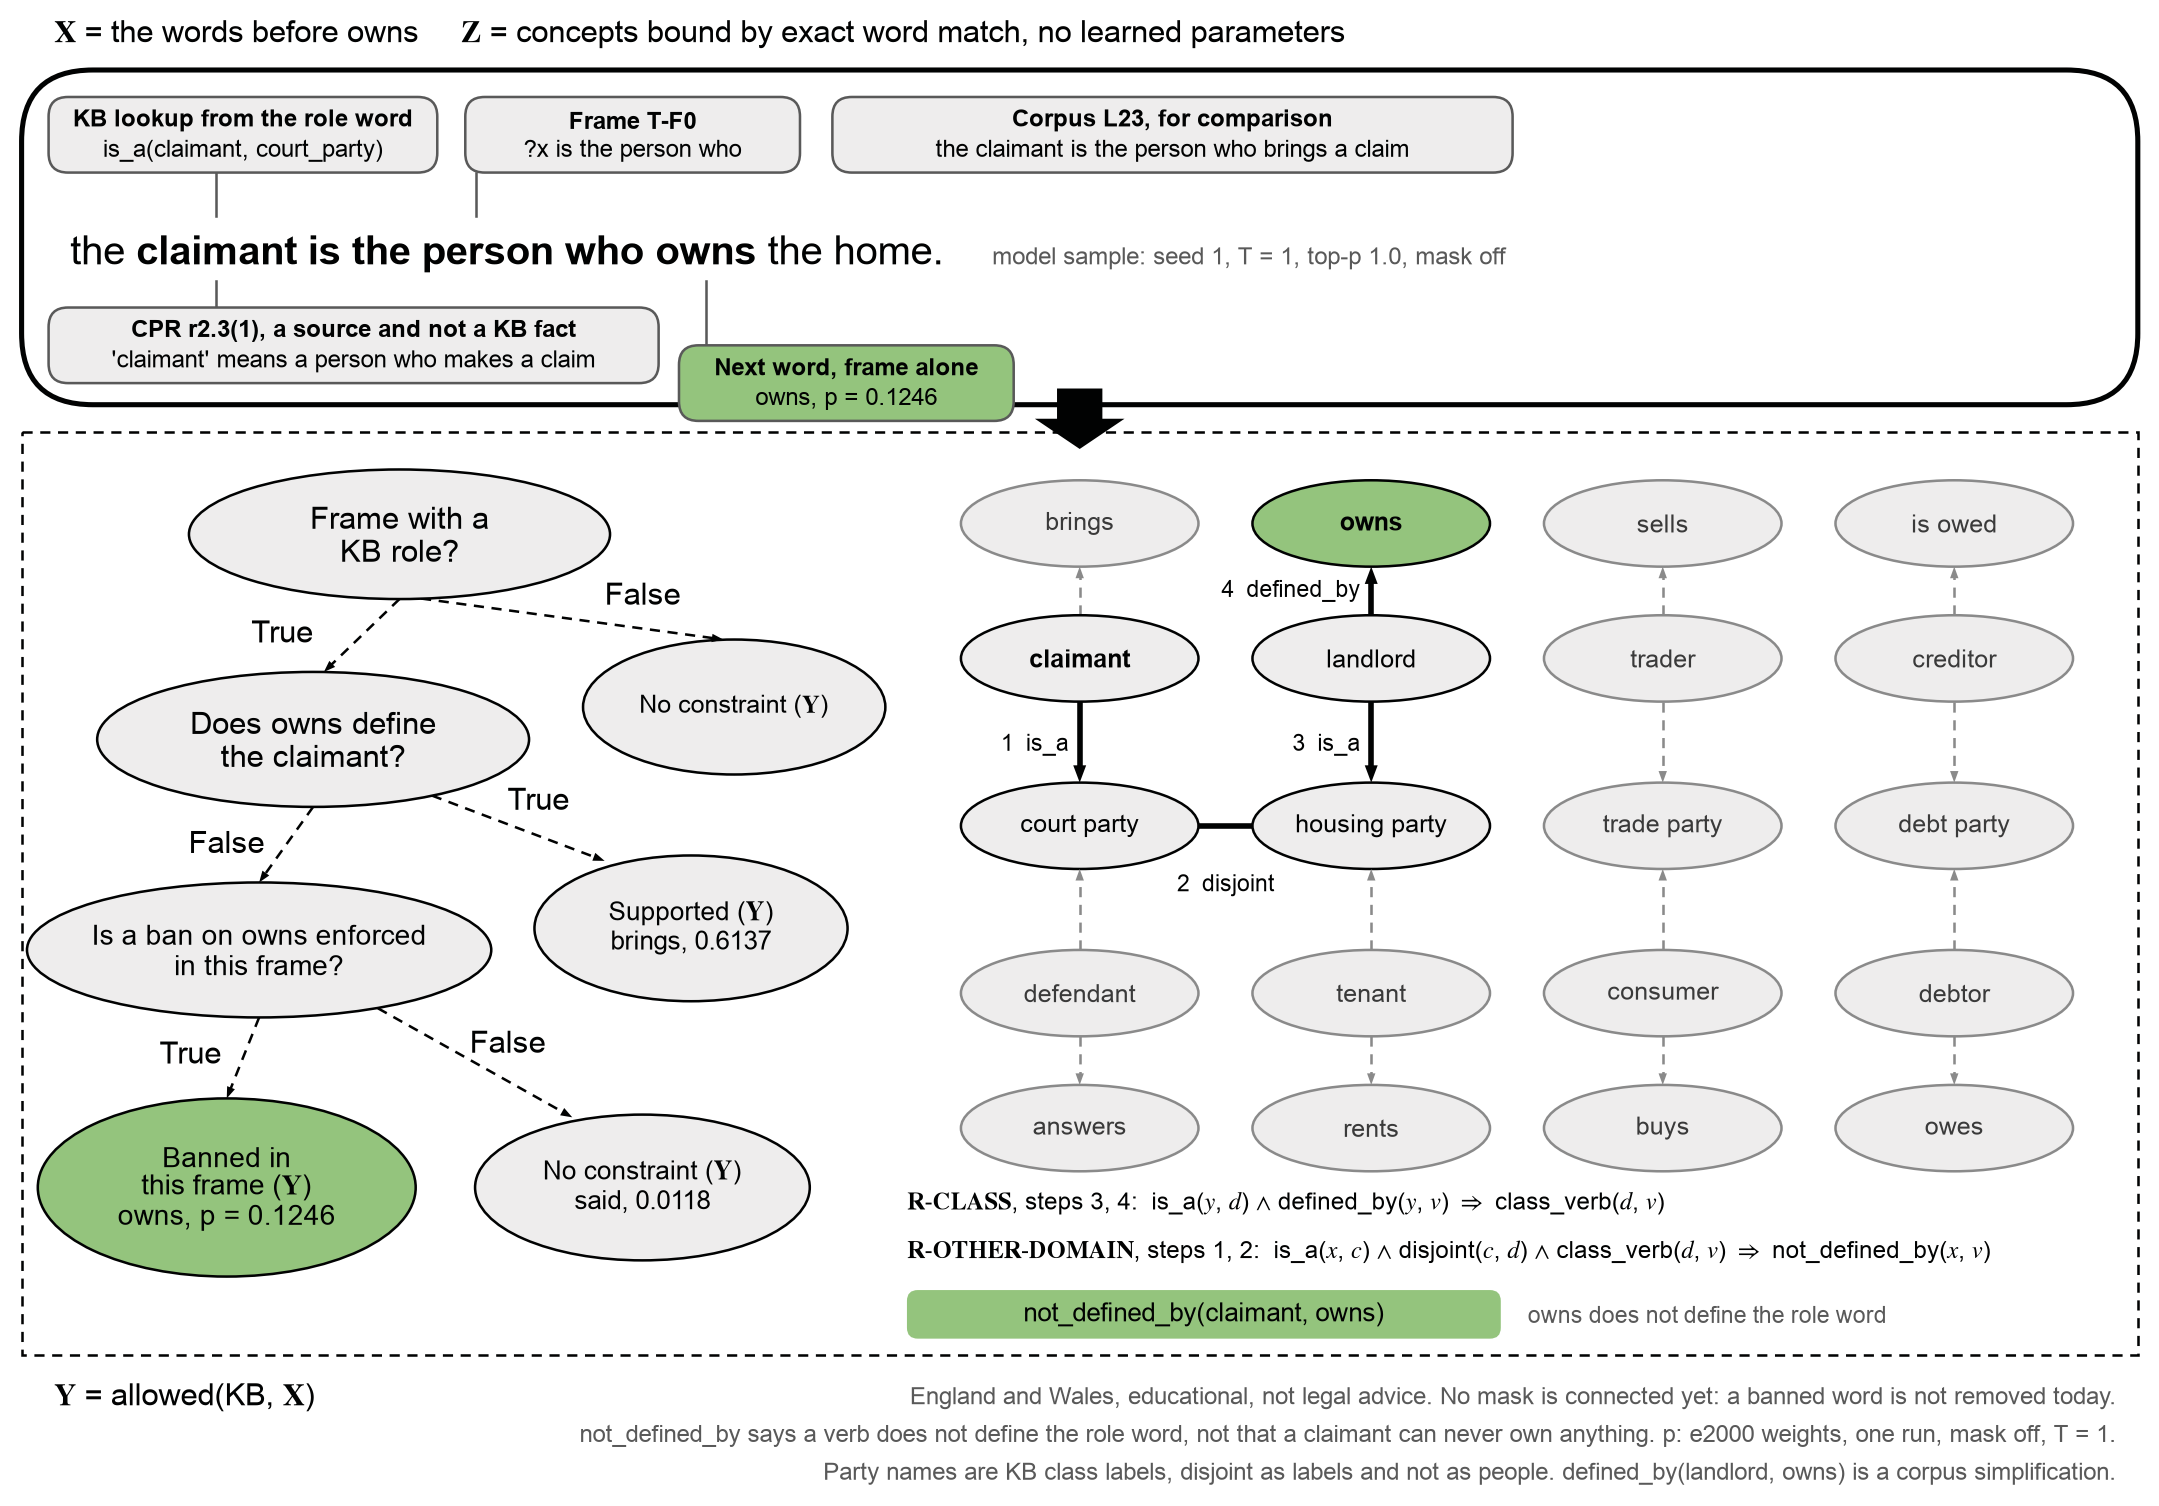
\includegraphics[width=\linewidth,trim=0 48 0 0,clip]{fig-civil-law-kb.png}\\[-2pt]
{\scriptsize\captionof{figure}{\textbf{The core logic.} After ``the claimant is the person who'', the network puts $p{=}0.1246$ on \emph{owns}; two KB rules derive \textit{not\_defined\_by}(claimant, owns), so \emph{owns} is banned and \emph{brings} is supported. $Y{=}\mathrm{allowed}(\mathrm{KB},X)$. One sample (seed 1, $T{=}1$, mask off); educational KB, not legal advice.}\label{fig:logic}}
\end{minipage}
\end{minipage}}\vspace{2pt}}
\makeatother

\title{\LARGE\bf Neural-Symbolic NLP on a Small Transformer:\\Towards Neurosymbolic World Models for Manipulation}

\author{\applicant\thanks{Research report for EPSRC DLA project S3.5-COM-Valentino, University of Sheffield, for Dr Marco Valentino (NLP group) and Dr Amir Ghalamzan. Live demo: \url{\demourl}. Code: \url{\codeurl}.}}

\begin{document}
\maketitle
\thispagestyle{empty}
\pagestyle{empty}

%======================================================================
\section{Introduction}
Foundation models give robots broad priors but no guarantee that a step obeys a rule. Vision-language-action (VLA) policies above 90\% success on standard LIBERO fall to 0.0\% under simple perturbations~\cite{liberopro}. On Towers of Hanoi, a PDDL-based neuro-symbolic system reached 95\% against 34\% for the best fine-tuned VLA~\cite{duggan}.

The same gap appears in language at a scale small enough to inspect. A transformer trained on next-token cross-entropy has no notion of truth: the loss rewards text that looks like the corpus. The baseline in this project reached a training loss of 0.2489, but by then its samples were copies of the training text, and earlier samples stated definitions the corpus does not contain, such as ``the claimant is the person who \emph{owns} the home'' (the corpus says \emph{brings a claim}).

Sheth et al.~\cite{sheth2023} frame the remedy as an integration of neural perception with symbolic knowledge, in two families. \emph{Lowering} compresses knowledge into the network, for example as embeddings or as masks on its inductive biases. \emph{Lifting} extracts neural outputs into symbols for reasoning, either through a decoupled pipeline or with neural and symbolic parts trained together. For mental-health assistance, they report 70\% expert satisfaction for an intertwined pipeline against 47\% for an LLM in a federated one; the process-knowledge line~\cite{sheth2022,roy2022} argues that such systems must follow, and explain themselves by, the expert's own guideline. On the lowering side, the semantic loss~\cite{xu2018} measures how far the network's output is from satisfying a logical constraint. The pseudo-semantic loss~\cite{ahmed2023} extends it to autoregressive models. On GPT-2, it was combined with word banning at decoding, which gave the lowest toxicity (9.20\%, against 9.80\% without banning and 14.05\% for domain-adaptive training alone).

This report asks: \emph{if one rule source is used in training, at decoding and to check the output, where does the constraint hold, and where does it fail?} Pairing constrained learning with constrained inference is published~\cite{ahmed2023}; what this project adds is a version small enough to trace every step. It contributes (i) a from-scratch transformer with a knowledge base (KB) used as a semantic loss, a hard logit mask and a verifier, (ii) a live demo that trains it in the browser, and (iii) measurements over four training seeds that separate trained from untrained contexts. \textbf{Try it:} the demo (Fig.~\ref{fig:demo}) takes one parameter line, for example \texttt{300 0.8 0.9 2 40 2 42}: epochs, temperature, top-$p$, layers, max tokens, $\lambda_s$ and seed.

%======================================================================
\section{Method}
\subsection{Model and corpus}
A decoder-only, pre-LayerNorm transformer~\cite{vaswani} is written in TypeScript without ML libraries: forward, backward, Adam and top-$p$ sampling, checked by finite-difference gradient tests. It has 2 layers, $d{=}32$, 2 heads, feed-forward width 128 and context 32, for 87,401 parameters. It trains on England \& Wales civil-dispute text (222 definitions and 34 stories; 937 whole-word BPE tokens), on all of it: there is no held-out text split.

\subsection{One knowledge base, two integration points}
The KB holds triples and Horn rules, closed once by forward chaining. For example, with $c$ the claimant and $d$ the defendant,
\[\begin{aligned}&\mathit{counterpart}(c,d)\wedge\mathit{defined\_by}(d,\mathrm{answers})\\&\qquad\Rightarrow\mathit{not\_defined\_by}(c,\mathrm{answers}),\end{aligned}\]
A trigger turns a derived fact into banned token IDs when the context ends in a definition frame such as ``the claimant is the person who'' (Fig.~\ref{fig:logic}). The KB yields one allowed set $A_t$ per position, used at two integration points, and the same facts check the output (Fig.~\ref{fig:pipe}):

\textbf{Training: semantic loss.} $\mathcal{L}=\mathrm{CE}+\lambda_s(-\log P_A)$, where $P_A$ is the probability mass on allowed tokens~\cite{xu2018,ahmed2023}. It acts only where a rule fires (86 of 85,984 training positions). It cannot see the choice among allowed tokens, since it depends on $P_A$ alone. Where data and rule conflict it is a soft penalty, with no test-time guarantee.

\textbf{Decoding: hard logit mask.} Banned logits are set to $-\infty$ before temperature and top-$p$. This guarantees zero mass on covered banned tokens, but only as far as the rules and triggers reach, and a wrong rule is enforced absolutely. The banned mass before masking ($\mathit{massBefore}$) is logged.

\textbf{Lifting: verifier and candidate facts.} A verifier parses generated text into triples and labels each claim \emph{supported}, \emph{contradicted} or \emph{unknown}. A probe reads confident predictions from the network as candidate facts (\emph{confirmed}, \emph{conflict} or \emph{novel}). They are reported, never added to the KB.

In the terms of~\cite{sheth2023} (our mapping), the mask is lowering by analogy, the semantic loss moves toward intertwined integration, and the verifier is decoupled lifting.

\begin{figure}[t]
\centering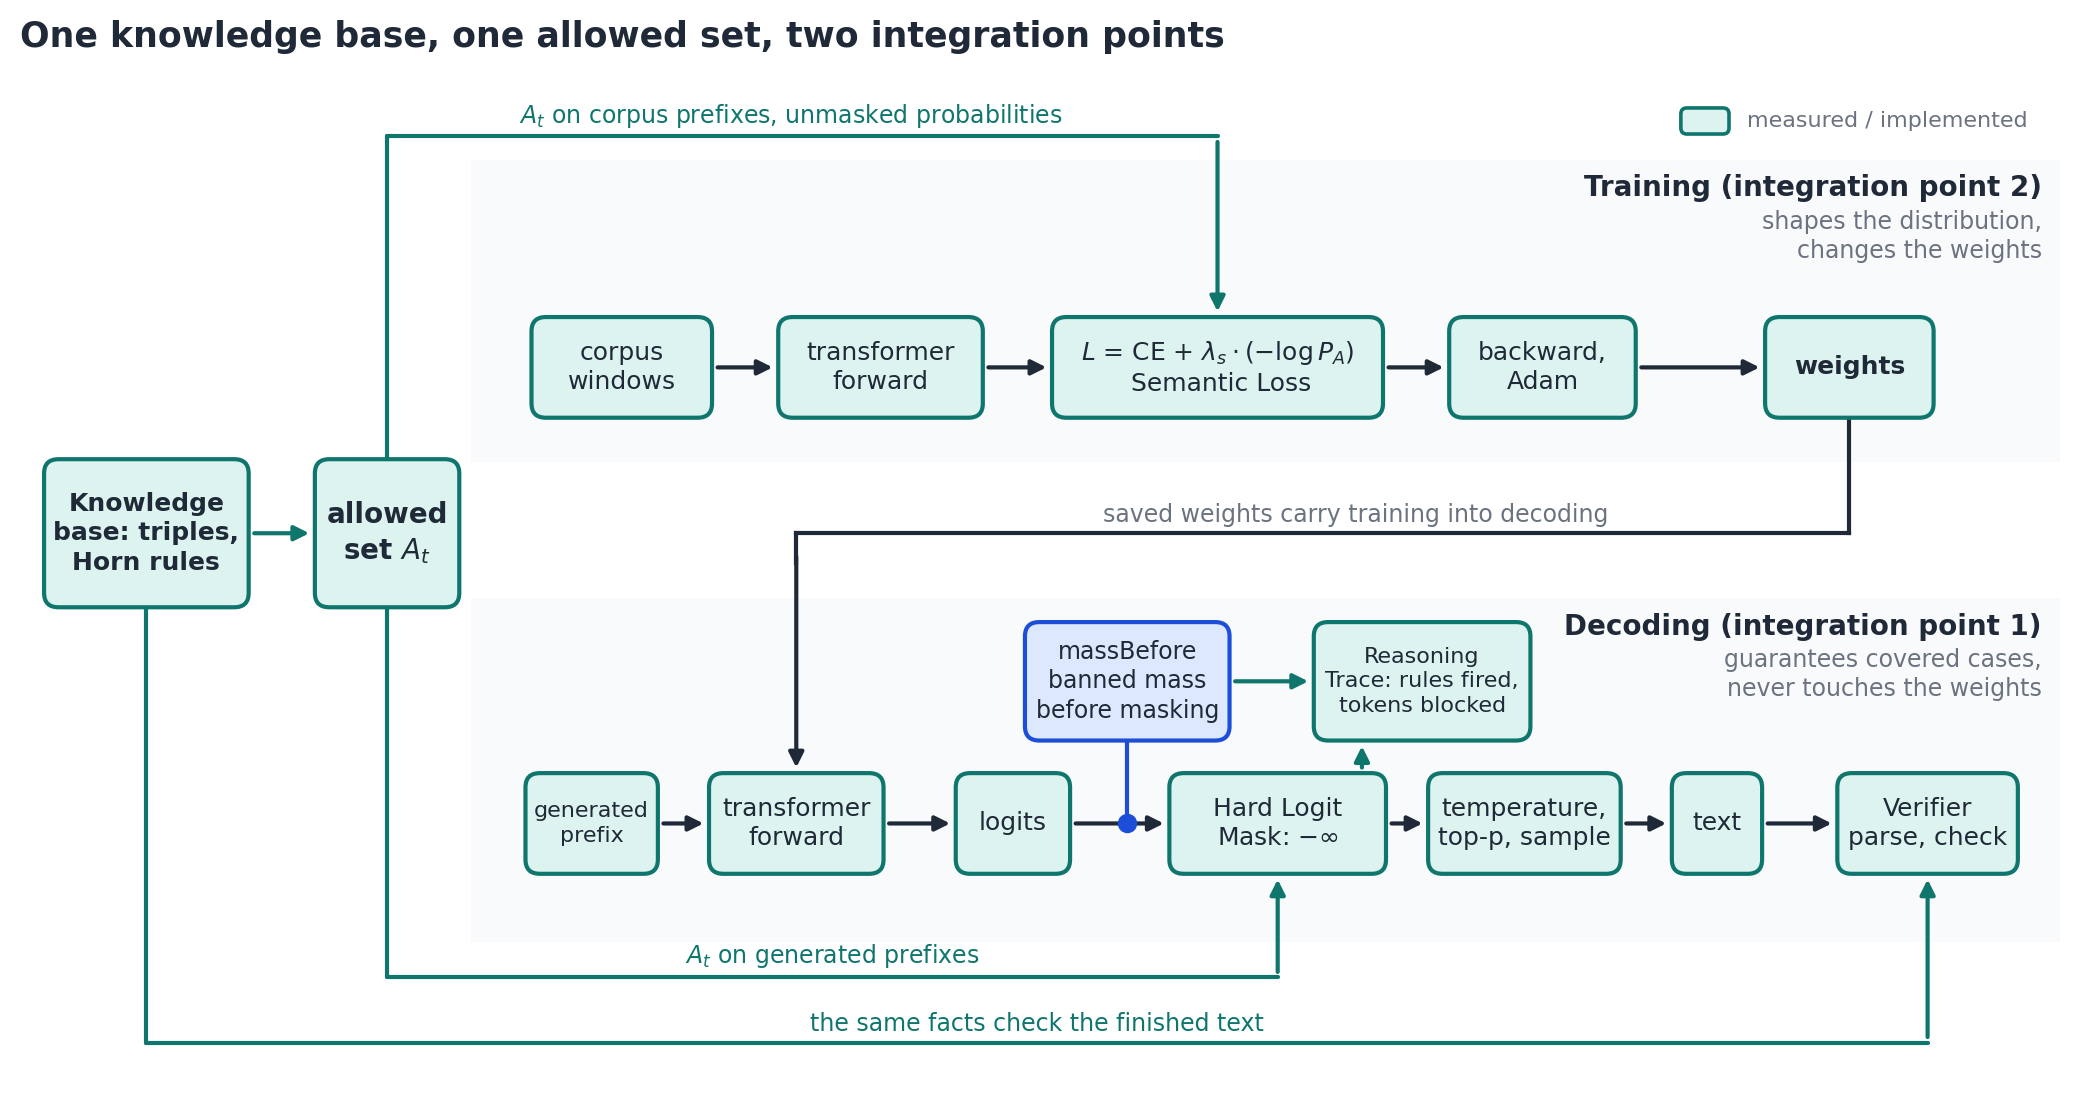
\includegraphics[width=\linewidth,trim=0 0 0 22,clip]{fig-design-pipeline.png}\vspace{-3pt}
\caption{One KB gives one allowed set $A_t$: the semantic loss uses it in training (weights), the hard mask at decoding (logits), and the verifier checks the finished text against the same facts.}\label{fig:pipe}
\end{figure}


\subsection{Protocol}
Prompts are every role in every definition frame, $8\times3=24$: 8 occur in the training text, and 16 put a role in a frame it never appears in (``the claimant is a business that''); these 16 are the only held-out data. Each prompt is sampled at seeds 0--49 for 20 tokens, at $T{=}0.8$, top-$p$ 0.9 and at $T{=}1$, top-$p$ 1, with the mask off and on. A rule counts as violated when its banned word's mean $p$ at its trigger is at least 0.02 (48 rules). All runs train for 2000 epochs: one run at $\lambda_s{=}50$ against the CE-only baseline (seed 42), and eight models at $\lambda_s\in\{0,2\}$ $\times$ seeds 42, 1, 2, 3. At seed 42, $\lambda_s{=}0$ reproduces the baseline's weights exactly.

%======================================================================
\section{Results}
\begin{figure*}[t]
\begin{minipage}[c]{0.60\textwidth}
\centering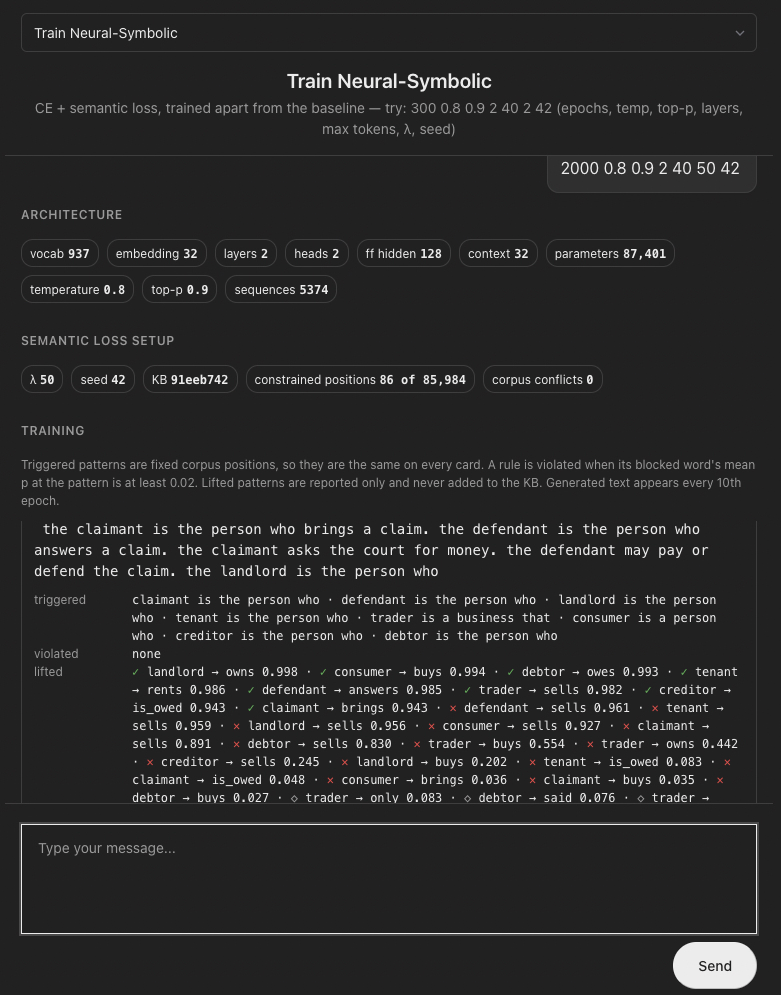
\includegraphics[height=5.4cm]{ns-l50-e2000-demo-epoch.png}\hspace{5pt}%
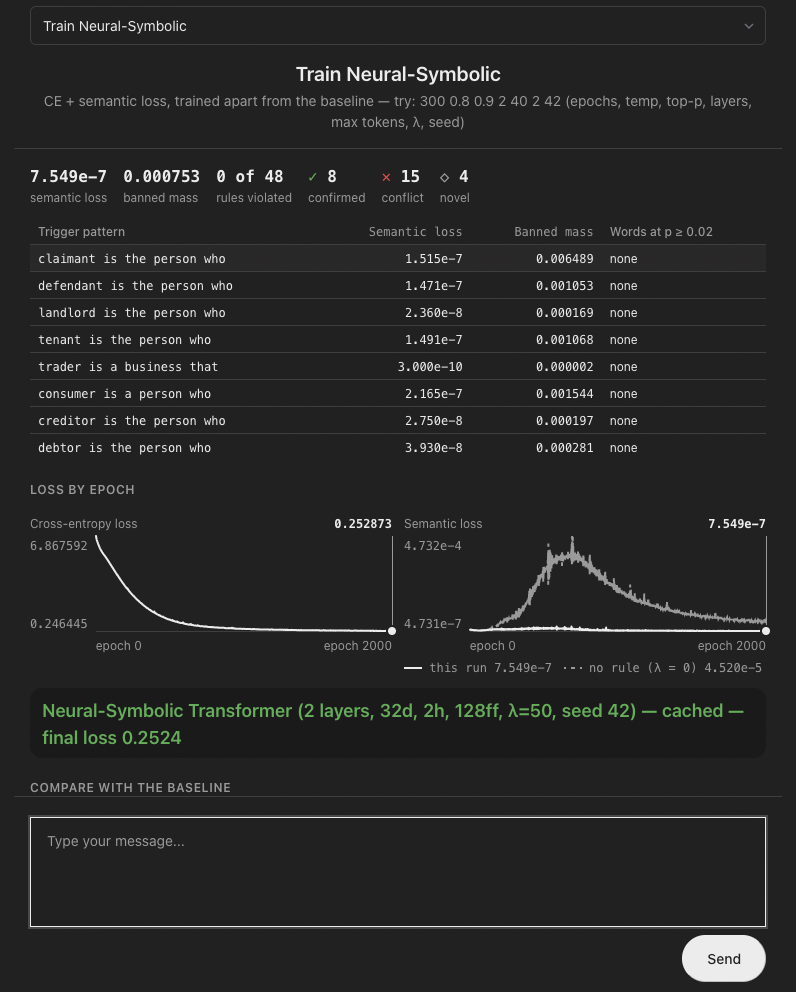
\includegraphics[height=5.4cm]{ns-l50-e2000-demo-dashboard.png}
\end{minipage}\hfill
\begin{minipage}[c]{0.37\textwidth}
\caption{\textbf{The live demo} after a 2000-epoch run at $\lambda_s{=}50$. Left: architecture, semantic-loss setup, generated text, the trigger patterns that fired and the facts lifted from the network. Right: semantic loss and banned mass for each of the 8 trigger patterns, 0 of 48 rules violated, and loss by epoch.\newline Live demo, try other settings:\newline \url{\demourl}\newline Code:\newline \url{\codeurl}}\label{fig:demo}
\end{minipage}
\end{figure*}

\subsection{One full-length run: $\lambda_s{=}50$ against CE only}
Table~\ref{tab:l50} reads the saved weights at the 86 positions where a rule fires. The banned mass is lower at every logged epoch (loss curves: Fig.~\ref{fig:demo}, right). Over all 2001 epochs, CE only violates a rule at 1846 of them; the constrained model at 175, and none after epoch 1746. Final training cross-entropy costs a little: 0.2524 against 0.2489.

\begin{table}[t]
\caption{Epoch 2000, seed 42, the 86 constrained training positions.}\label{tab:l50}
\centering\footnotesize\setlength{\tabcolsep}{4pt}
\begin{tabular}{@{}lrr@{}}
\toprule
Measure & CE only & CE + sem.\ loss\\
\midrule
Semantic loss & 4.58e-5 & 6.26e-7\\
Banned mass & 0.0419 & 0.0006\\
$p$(next corpus word) & 0.946 & 0.978\\
$p$(role's own verb) & 0.809 & 0.841\\
Rules violated (of 48) & 7 & 0\\
Training cross-entropy & 0.2489 & 0.2524\\
\bottomrule
\end{tabular}
\end{table}


\subsection{Trained and untrained contexts}
With the mask off, the $\lambda_s{=}50$ model made no contradicted claim in 1,173 on the 8 training-text prompts (CE only: 1.2\% at $T{=}0.8$, 4.8\% at $T{=}1$). On the 16 untrained prompts it still contradicts the KB in 35--36\% of claims, against 41--43\% for CE only. Of its 430 contradicted claims at $T{=}0.8$, 315 are ``sells'' after ``is a business that'' (the verb of \emph{trader}, the one role trained in that frame) and 100 are ``buys'' after ``is a person who'' (the verb of \emph{consumer}). Both models complete a frame with the verb of the role trained in it, whatever the role: the frame, not the role, appears to drive the prediction (not yet tested separately). With the mask on, the banned verb's replacement is mostly one the KB knows nothing about (CE only: \emph{unknown} claims rise from 50 to 443).

\subsection{Four training seeds}
Table~\ref{tab:e4} compares $\lambda_s{=}2$ with $\lambda_s{=}0$. With 4 of 4 seeds in one direction a paired sign-flip test cannot go below $p{=}0.125$, so ``at every seed'' is not a significance claim.

\begin{table}[t]
\caption{Seeds 42, 1, 2, 3, $\lambda_s{=}0$ vs 2, mask off; ranges over seeds or seed pairs.}\label{tab:e4}
\centering\footnotesize\setlength{\tabcolsep}{3pt}
\begin{tabular}{@{}lrr@{}}
\toprule
Measure & $\lambda_s{=}0$ & $\lambda_s{=}2$\\
\midrule
Banned mass, 86 constrained pos. & 0.024--0.049 & 0.008--0.016\\
Banned mass, 16 untrained prompts & 0.45--0.73 & 0.43--0.71\\
Contradicted, untrained, $T{=}0.8$ & 35.4--47.9\% & 31.3--45.7\%\\
JS of $(P_A,1{-}P_A)$, mean & 7.5e-3 & 2.5e-3\\
JS of $q_A$ (among allowed), mean & 0.0153 & 0.0149\\
Weight cosine between seeds & 0.023--0.071 & 0.025--0.071\\
Same top-1 word, held-out prompts & 58\% & 61\%\\
Perplexity, no rule fires (train) & 1.266--1.283 & 1.264--1.281\\
\bottomrule
\end{tabular}
\end{table}

\textbf{Seeds (E1).} At $\lambda_s{=}0$, final training loss is similar (0.2358--0.2489) but weights are close to unrelated (cosine 0.023--0.071). All four seeds pick the same next word on every training-text prompt, but on held-out prompts only 50--69\% of the time.

\textbf{Semantic loss (E4).} Banned mass at the constrained positions is 2.6--4.3$\times$ lower at every seed. Seeds disagree three times less on how much mass goes to allowed words, while their disagreement \emph{among} allowed words is unchanged, as predicted. Perplexity where no rule fires does not rise (training text only). On untrained prompts the effect is small: banned mass falls by 0.02--0.13 and contradicted claims by 2--9 points.

\textbf{Mask coverage.} With the mask on, 514 of 23,664 parsed claims still contradict the KB. All are one surface form, ``that \emph{owed} money'': the verifier reads it as \emph{is owed}, but the mask bans ``owed'' only after ``is''. This is a mask--verifier coverage gap, not a model property.

%======================================================================
\section{Conclusion}
Three findings hold across seeds. \textbf{Where the constraint is trained, it holds}, at a small cost in training loss. \textbf{Beyond it, the rule does not transfer}: on unseen frames the model follows the frame, not the KB. \textbf{A guarantee covers only what its rules cover}, as the ``owed'' gap shows. Limits: one small model, a hand-written KB, four seeds, and no held-out text or KB yet.

\textbf{The same principle on any LLM.} Sheth et al.~\cite{sheth2023} call systems in which an LLM hands sub-tasks to symbolic solvers \emph{federated pipelines}. Here the KB is the solver, and the three access points of Fig.~\ref{fig:pipe} become three levels of API access. With open weights, the semantic loss applies in fine-tuning. Where an API exposes logits or a logit bias, the allowed set can mask decoding. With text only, the verifier returns contradicted claims for regeneration, the verify-and-refine loop of Explanation-Refiner~\cite{quan2024,quan2025} and LLM-Modulo~\cite{llmmodulo}. This extension is designed, not built.


\textbf{Towards neurosymbolic world models.} The PhD carries the same split to manipulation. Tokens become actions and states, and the allowed set becomes PDDL preconditions, effects and contact constraints such as bounds on predicted slip. The loss trains the world model, the mask rejects actions, and the verifier checks before execution and triggers recovery. \emph{O1, foundations (Years 1--2):} a multimodal model proposes PDDL action models under training and decoding constraints~\cite{xu2018,ahmed2023}. Their semantic faithfulness, not just syntax, is checked by prover-based verification~\cite{quan2024,quan2025}; GPT-4o's PDDL was 96.1\% parseable but 24.8\% correct~\cite{planetarium}. O1 also tests whether world models follow plausibility over validity, like the frame effect above, and whether steering or circuit methods~\cite{valentino2026,kim2025} reduce it. \emph{O2, multi-timescale control (Years 2--3):} a slow symbolic layer sets subgoals and constraints. A fast controller rolls out an action-conditioned tactile model~\cite{mandil,nazari2022} and checks constraints on predicted states, so a predicted violation triggers replanning before failure, compared with post-failure recovery~\cite{reflect}. Evaluation moves from simulation to tactile hardware, against VLA and LLM-planner baselines~\cite{liberopro,duggan}. The main risk is the one the demo exposed: a wrong or missing rule enters training and decoding at once. So every rule stays traceable to a proof, and where formalisation fails the verifier says \emph{unknown}.

\begin{thebibliography}{99}
\scriptsize
\setlength{\itemsep}{0pt}
\bibitem{liberopro} X.~Zhou \emph{et al.}, ``LIBERO-PRO: Towards robust and fair evaluation of vision-language-action models beyond memorization,'' arXiv:2510.03827, 2025.
\bibitem{duggan} T.~Duggan \emph{et al.}, ``The price is not right: Neuro-symbolic methods outperform VLAs on structured long-horizon manipulation tasks,'' in \emph{Proc. ICRA}, 2026.
\bibitem{sheth2023} A.~Sheth, K.~Roy, and M.~Gaur, ``Neurosymbolic artificial intelligence (why, what, and how),'' \emph{IEEE Intell. Syst.}, vol.~38, no.~3, pp.~56--62, 2023.
\bibitem{sheth2022} A.~Sheth, M.~Gaur, K.~Roy, R.~Venkataraman, and V.~Khandelwal, ``Process knowledge-infused AI: Towards user-level explainability, interpretability, and safety,'' arXiv:2206.13349, 2022.
\bibitem{roy2022} K.~Roy, M.~Gaur, Q.~Zhang, and A.~Sheth, ``Process knowledge-infused learning for suicidality assessment on social media,'' arXiv:2204.12560, 2022.
\bibitem{xu2018} J.~Xu, Z.~Zhang, T.~Friedman, Y.~Liang, and G.~Van den Broeck, ``A semantic loss function for deep learning with symbolic knowledge,'' in \emph{Proc. ICML}, 2018.
\bibitem{ahmed2023} K.~Ahmed, K.-W.~Chang, and G.~Van den Broeck, ``A pseudo-semantic loss for autoregressive models with logical constraints,'' in \emph{Proc. NeurIPS}, 2023.
\bibitem{vaswani} A.~Vaswani \emph{et al.}, ``Attention is all you need,'' in \emph{Proc. NeurIPS}, 2017.
\bibitem{quan2024} X.~Quan, M.~Valentino, L.~A.~Dennis, and A.~Freitas, ``Verification and refinement of natural language explanations through LLM-symbolic theorem proving,'' in \emph{Proc. EMNLP}, 2024.
\bibitem{quan2025} X.~Quan, M.~Valentino, L.~A.~Dennis, and A.~Freitas, ``Faithful and robust LLM-driven theorem proving for NLI explanations,'' in \emph{Proc. ACL}, 2025.
\bibitem{llmmodulo} S.~Kambhampati \emph{et al.}, ``LLMs can't plan, but can help planning in LLM-Modulo frameworks,'' in \emph{Proc. ICML}, 2024.
\bibitem{planetarium} M.~Zuo \emph{et al.}, ``Planetarium: A rigorous benchmark for translating text to structured planning languages,'' in \emph{Proc. NAACL}, 2025.
\bibitem{valentino2026} M.~Valentino, G.~Kim, D.~Dalal, Z.~Zhao, and A.~Freitas, ``Mitigating content effects on reasoning in language models through fine-grained activation steering,'' in \emph{Proc. AAAI}, 2026.
\bibitem{kim2025} G.~Kim, M.~Valentino, and A.~Freitas, ``Reasoning circuits in language models: A mechanistic interpretation of syllogistic inference,'' in \emph{Findings of ACL}, 2025.
\bibitem{mandil} W.~Mandil, K.~Nazari, and A.~Ghalamzan~E, ``Action conditioned tactile prediction: A case study on slip prediction,'' arXiv:2205.09430, 2022.
\bibitem{nazari2022} K.~Nazari, W.~Mandil, and A.~Ghalamzan~E, ``Proactive slip control by learned slip model and trajectory adaptation,'' arXiv:2209.06019, 2022.
\bibitem{reflect} Z.~Liu, A.~Bahety, and S.~Song, ``REFLECT: Summarizing robot experiences for failure explanation and correction,'' in \emph{Proc. CoRL}, 2023.
\end{thebibliography}

\end{document}
